\section{Feature definitions}\label{app:features}

\begin{table}[H]
\centering\caption{Feature definitions}\label{tab:features}
\footnotesize
\begin{tabular}{>{\raggedright\arraybackslash}p{4.4cm}>{\raggedright\arraybackslash}p{2.1cm}p{8.4cm}}
\toprule
Feature & Set & Definition (bar $t$; $r$ log return, $V$ volume, $B$ taker-buy volume, $C,H,L,O$ prices)\\
\midrule
\multicolumn{3}{l}{\emph{Spread and price impact}}\\
cs\_spread\_24 & MS$_{\text{proxy}}$ & 24h mean of the two-bar \citet{corwin2012} estimator\\
ar\_spread\_24 & MS$_{\text{proxy}}$ & $\sqrt{\max(0,\overline{4(c_{t-1}-\eta_{t-1})(c_{t-1}-\eta_t)})}$ over 24h, $\eta=(\log H+\log L)/2$ \citep{abdi2017}\\
roll\_spread\_48 & MS$_{\text{proxy}}$ & $2\sqrt{\max(0,-\operatorname{cov}(r_t,r_{t-1}))}$ over 48h \citep{roll1984}\\
amihud\_24 & MS$_{\text{proxy}}$ & log of 24h mean of $|r_t|/(C_tV_t)$ \citep{amihud2002}\\
sqrt\_impact\_24 & MS$_{\text{proxy}}$ & log of 24h mean of $|r_t|/\sqrt{V_t/\bar V_{168}}$\\
\multicolumn{3}{l}{\emph{Order flow, BVC proxy (signed volume $S_t=(2\Phi(r_t/\hat\sigma_{168})-1)V_t$)}}\\
ofi\_1, ofi\_24 & MS$_{\text{proxy}}$, Flow$_{\text{BVC}}$ & $S_t/\bar V_{168}$; $\sum_{24}S/\sum_{24}V$\\
ofi\_accel & MS$_{\text{proxy}}$, Flow$_{\text{BVC}}$ & 6h imbalance minus 24h imbalance\\
vpin\_24 & MS$_{\text{proxy}}$, Flow$_{\text{BVC}}$ & $\sum_{24}|S|/\sum_{24}V$\\
kyle\_lambda\_48 & MS$_{\text{proxy}}$, Flow$_{\text{BVC}}$ & $\operatorname{cov}(r,SC)/\operatorname{var}(SC)$ over 48h\\
\multicolumn{3}{l}{\emph{Order flow, observed (signed volume $2B_t-V_t$) and trade activity}}\\
taker\_imb\_1, \_24, \_accel, taker\_vpin\_24, kyle\_lambda\_true\_48 & MS, Flow$_{\text{taker}}$ & as the BVC versions, with observed signed volume\\
taker\_imb\_late15 & MS & taker imbalance in minutes 45--59 of the hour\\
trades\_z\_168, trade\_size\_z\_168 & MS & 168h z-scores of log trade count and log average dollar trade size\\
\multicolumn{3}{l}{\emph{Volatility}}\\
gk\_vol\_24, rs\_vol\_24, yz\_vol\_24 & MS$_{\text{proxy}}$ & log 24h \citet{garman1980}, \citet{rogers1991}, \citet{yang2000} volatility\\
vol\_ratio\_24\_168 & MS$_{\text{proxy}}$ & log ratio of 24h to 168h Garman-Klass volatility\\
vol\_of\_vol\_168 & MS$_{\text{proxy}}$ & 168h standard deviation of log 24h Garman-Klass volatility\\
rv\_1m\_1, rv\_1m\_24 & MS & log realised variance from 1-minute returns, current hour and 24h\\
jump\_share\_24 & MS & 24h mean of $\max(RV-BV,0)/RV$ \citep{bns2004}\\
rskew\_24 & MS & 24h mean of hourly realised skewness \citep{amaya2015}\\
\multicolumn{3}{l}{\emph{Efficiency, bar structure, activity}}\\
eff\_ratio\_24 & MS$_{\text{proxy}}$ & $|\log C_t-\log C_{t-24}|/\sum_{24}|r|$\\
autocorr\_48 & MS$_{\text{proxy}}$ & 48h first-order autocorrelation of $r$\\
var\_ratio\_4\_168 & MS$_{\text{proxy}}$ & variance of 4h returns over 4 times variance of 1h returns, 168h\\
body\_share, upper\_wick, lower\_wick (24h) & MS$_{\text{proxy}}$ & candle body and wicks as share of the high-low range\\
volume\_z\_168, volume\_trend\_24\_168 & MS$_{\text{proxy}}$ & z-score of log volume; log ratio of 24h to 168h mean volume\\
\multicolumn{3}{l}{\emph{Technical controls}}\\
mom\_1, \_4, \_24, \_168 & TI & $\log C_t-\log C_{t-k}$\\
rsi\_14, macd\_hist, bb\_pctb\_20 & TI & RSI(14); MACD(12,26,9) histogram over price; Bollinger \%B(20,2)\\
ma\_gap\_24, ma\_gap\_168, atr\_14 & TI & log gap to moving average; ATR(14) over price\\
\bottomrule
\end{tabular}
\end{table}

\section{Leakage controls and a positive control}\label{app:leakage}

The replication package contains automated tests that run in a few seconds.
(i) \emph{Causality of features}: for three cut-off dates, every bar after the cut-off is multiplied
by random noise and every feature at or before the cut-off is recomputed; the test fails if any
value changes. The same test is applied to the intrahour features built from one-minute bars.
(ii) \emph{Target definition}: $y_t$ must equal $\log C_{t+h}-\log C_t$ exactly.
(iii) \emph{Purging}: for every fold and every horizon, the last training label must be observed
before the first test bar, and the same must hold for the inner validation split.
(iv) \emph{Analyses}: every validation and robustness function is run on synthetic data and checked
for internal consistency (for example, the in-sample ceiling must weakly exceed the squared
correlation of BVC), a pure-noise predictor must not produce an out-of-sample gain in the
single-predictor walk-forward, and a planted flow signal must be recovered from observed flow but
not from technical momentum.

As a positive control we run the full pipeline on a synthetic two-year hourly series with GARCH-type
volatility, in which a persistent latent order flow drives the taker share of volume and each hour's
return loads negatively on the average flow of the previous four hours. The contemporaneous link
between flow and the bar's return is deliberately weak, so BVC recovers the flow only poorly, as in
the real data. The pipeline should find the
signal with observed-flow features and much less of it with BVC features, and nothing with technical
indicators. It does: the observed-flow elastic net reaches an out-of-sample $R^2$ of about 3\% with a
Clark-West $t$-statistic above 10, the BVC-flow model about zero, and the technical model a negative
$R^2$. A pipeline that leaked future information would instead show gains for every feature set. The
script \texttt{scripts/make\_synthetic.py} generates the series.

\section{Zero-fee experiment: robustness}\label{app:fee}

\begin{table}[H]
\centering\caption{Effects of removing and restoring fees: alternative specifications}\label{tab:feerobust}
\resizebox{\textwidth}{!}{\begin{tabular}{lrrrrrr}
\toprule
 & \multicolumn{4}{c}{Event windows} & \multicolumn{2}{c}{Full windows}\\
\cmidrule(lr){2-5}\cmidrule(lr){6-7}Measure & Main (90 days) & ETH only & 60 days & 180 days & Means & With trend\\
\midrule
\multicolumn{7}{l}{\emph{Panel A. Fees removed (8 July 2022)}}\\
Trades per day (millions) & 1.68 (12.2) & 1.25 (11.0) & 1.53 (10.1) & 2.04 (14.7) & 2.14 (16.0) & 1.58 (9.7)\\
Dollar volume per day (\$bn) & 1.21 (5.9) & 1.03 (4.4) & 0.90 (6.6) & 1.62 (9.5) & 1.77 (10.5) & 1.09 (4.8)\\
Average trade size (\$) & \ensuremath{-}0.46 (\ensuremath{-}4.3) & \ensuremath{-}0.22 (\ensuremath{-}1.4) & \ensuremath{-}0.63 (\ensuremath{-}10.4) & \ensuremath{-}0.41 (\ensuremath{-}6.5) & \ensuremath{-}0.37 (\ensuremath{-}6.7) & \ensuremath{-}0.49 (\ensuremath{-}4.6)\\
Directional volume $\sum_m|B_m-S_m|$ (\$bn) & 0.43 (3.3) & 0.25 (1.4) & 0.21 (2.6) & 0.72 (5.7) & 0.85 (6.4) & 0.29 (2.0)\\
Two-sided volume (\$bn) & 1.43 (6.0) & 1.22 (4.9) & 1.09 (6.1) & 1.91 (9.5) & 2.04 (11.1) & 1.34 (4.8)\\
Two-sided share of volume & 0.16 (6.2) & 0.15 (8.6) & 0.14 (4.7) & 0.20 (9.9) & 0.19 (12.0) & 0.18 (4.7)\\
Mean $|$hourly taker imbalance$|$ & \ensuremath{-}1.03 (\ensuremath{-}9.3) & \ensuremath{-}0.86 (\ensuremath{-}7.3) & \ensuremath{-}0.98 (\ensuremath{-}6.9) & \ensuremath{-}1.22 (\ensuremath{-}12.8) & \ensuremath{-}1.25 (\ensuremath{-}16.1) & \ensuremath{-}1.07 (\ensuremath{-}6.2)\\
Amihud ratio, hourly bars ($|r|$ per \$bn) & \ensuremath{-}1.18 (\ensuremath{-}6.9) & \ensuremath{-}1.20 (\ensuremath{-}5.8) & \ensuremath{-}0.93 (\ensuremath{-}7.0) & \ensuremath{-}1.81 (\ensuremath{-}8.6) & \ensuremath{-}1.96 (\ensuremath{-}10.3) & \ensuremath{-}0.98 (\ensuremath{-}5.1)\\
Kyle's $\lambda$, BVC-signed flow (bps per \$M) & \ensuremath{-}0.39 (\ensuremath{-}3.1) & \ensuremath{-}0.52 (\ensuremath{-}3.0) & \ensuremath{-}0.22 (\ensuremath{-}2.2) & \ensuremath{-}0.99 (\ensuremath{-}5.2) & \ensuremath{-}1.14 (\ensuremath{-}6.3) & \ensuremath{-}0.29 (\ensuremath{-}1.7)\\
VPIN, BVC & \ensuremath{-}0.10 (\ensuremath{-}4.7) & \ensuremath{-}0.08 (\ensuremath{-}3.5) & \ensuremath{-}0.08 (\ensuremath{-}3.7) & \ensuremath{-}0.11 (\ensuremath{-}5.7) & \ensuremath{-}0.11 (\ensuremath{-}6.4) & \ensuremath{-}0.06 (\ensuremath{-}2.0)\\
Kyle's $\lambda$, observed flow (bps per \$M) & 0.24 (1.4) & \ensuremath{-}0.03 (\ensuremath{-}0.2) & 0.35 (1.8) & \ensuremath{-}0.22 (\ensuremath{-}1.2) & \ensuremath{-}0.29 (\ensuremath{-}1.7) & 0.30 (1.4)\\
VPIN, observed flow & \ensuremath{-}1.08 (\ensuremath{-}8.8) & \ensuremath{-}0.90 (\ensuremath{-}7.2) & \ensuremath{-}1.01 (\ensuremath{-}6.9) & \ensuremath{-}1.26 (\ensuremath{-}12.2) & \ensuremath{-}1.29 (\ensuremath{-}15.4) & \ensuremath{-}1.11 (\ensuremath{-}6.0)\\
$R^2$ of 1m returns on observed flow & 0.13 (5.2) & 0.08 (3.1) & 0.11 (4.5) & 0.14 (7.5) & 0.17 (8.1) & 0.10 (3.1)\\
corr(BVC, observed imbalance), 1m & 0.05 (4.1) & 0.00 (0.2) & 0.04 (2.7) & 0.08 (6.2) & 0.10 (6.6) & 0.03 (1.6)\\
Realised volatility (\% per day) & 0.15 (1.4) & \ensuremath{-}0.28 (\ensuremath{-}2.4) & 0.11 (0.9) & \ensuremath{-}0.26 (\ensuremath{-}1.6) & \ensuremath{-}0.22 (\ensuremath{-}1.6) & 0.25 (1.3)\\
First-order autocorrelation of 1m returns & \ensuremath{-}0.01 (\ensuremath{-}0.5) & \ensuremath{-}0.01 (\ensuremath{-}1.7) & \ensuremath{-}0.02 (\ensuremath{-}2.5) & 0.01 (1.2) & 0.00 (0.4) & 0.00 (\ensuremath{-}0.2)\\
\midrule
\multicolumn{7}{l}{\emph{Panel B. Fees restored (22 March 2023)}}\\
Trades per day (millions) & \ensuremath{-}1.68 (\ensuremath{-}18.1) & \ensuremath{-}1.84 (\ensuremath{-}31.7) & \ensuremath{-}1.70 (\ensuremath{-}16.0) & \ensuremath{-}1.71 (\ensuremath{-}16.2) & \ensuremath{-}1.59 (\ensuremath{-}13.5) & \ensuremath{-}2.12 (\ensuremath{-}12.6)\\
Dollar volume per day (\$bn) & \ensuremath{-}1.18 (\ensuremath{-}11.2) & \ensuremath{-}1.56 (\ensuremath{-}33.1) & \ensuremath{-}1.26 (\ensuremath{-}11.7) & \ensuremath{-}1.26 (\ensuremath{-}10.9) & \ensuremath{-}1.09 (\ensuremath{-}7.7) & \ensuremath{-}1.74 (\ensuremath{-}9.0)\\
Average trade size (\$) & 0.50 (7.5) & 0.28 (4.6) & 0.44 (10.3) & 0.45 (8.9) & 0.50 (9.8) & 0.38 (5.4)\\
Directional volume $\sum_m|B_m-S_m|$ (\$bn) & \ensuremath{-}0.27 (\ensuremath{-}3.1) & \ensuremath{-}0.59 (\ensuremath{-}11.2) & \ensuremath{-}0.36 (\ensuremath{-}4.0) & \ensuremath{-}0.24 (\ensuremath{-}2.8) & \ensuremath{-}0.13 (\ensuremath{-}1.5) & \ensuremath{-}0.67 (\ensuremath{-}5.2)\\
Two-sided volume (\$bn) & \ensuremath{-}1.33 (\ensuremath{-}12.0) & \ensuremath{-}1.79 (\ensuremath{-}30.8) & \ensuremath{-}1.38 (\ensuremath{-}11.4) & \ensuremath{-}1.48 (\ensuremath{-}10.7) & \ensuremath{-}1.30 (\ensuremath{-}7.5) & \ensuremath{-}1.96 (\ensuremath{-}8.5)\\
Two-sided share of volume & \ensuremath{-}0.15 (\ensuremath{-}8.9) & \ensuremath{-}0.18 (\ensuremath{-}9.5) & \ensuremath{-}0.13 (\ensuremath{-}11.4) & \ensuremath{-}0.19 (\ensuremath{-}9.2) & \ensuremath{-}0.18 (\ensuremath{-}8.4) & \ensuremath{-}0.19 (\ensuremath{-}6.1)\\
Mean $|$hourly taker imbalance$|$ & 1.15 (21.3) & 1.18 (19.5) & 1.08 (22.3) & 1.26 (18.9) & 1.16 (13.5) & 1.33 (9.8)\\
Amihud ratio, hourly bars ($|r|$ per \$bn) & 1.52 (21.8) & 1.77 (20.7) & 1.49 (38.8) & 1.39 (18.2) & 1.16 (8.3) & 2.09 (11.6)\\
Kyle's $\lambda$, BVC-signed flow (bps per \$M) & 0.97 (15.2) & 1.14 (17.4) & 0.98 (13.6) & 0.90 (12.0) & 0.70 (5.9) & 1.51 (10.2)\\
VPIN, BVC & 0.11 (5.1) & 0.07 (2.6) & 0.10 (4.8) & 0.08 (3.4) & 0.07 (2.8) & 0.11 (4.1)\\
Kyle's $\lambda$, observed flow (bps per \$M) & 0.30 (4.1) & 0.65 (5.9) & 0.24 (6.0) & 0.19 (2.2) & 0.09 (1.0) & 0.65 (3.8)\\
VPIN, observed flow & 1.11 (23.1) & 1.14 (25.1) & 1.04 (31.0) & 1.23 (19.6) & 1.13 (13.3) & 1.29 (9.8)\\
$R^2$ of 1m returns on observed flow & \ensuremath{-}0.06 (\ensuremath{-}3.8) & \ensuremath{-}0.03 (\ensuremath{-}1.3) & \ensuremath{-}0.08 (\ensuremath{-}6.8) & \ensuremath{-}0.04 (\ensuremath{-}1.7) & \ensuremath{-}0.01 (\ensuremath{-}0.7) & \ensuremath{-}0.08 (\ensuremath{-}2.6)\\
corr(BVC, observed imbalance), 1m & \ensuremath{-}0.05 (\ensuremath{-}6.2) & \ensuremath{-}0.04 (\ensuremath{-}3.3) & \ensuremath{-}0.04 (\ensuremath{-}7.8) & \ensuremath{-}0.03 (\ensuremath{-}2.2) & \ensuremath{-}0.01 (\ensuremath{-}0.4) & \ensuremath{-}0.07 (\ensuremath{-}3.5)\\
Realised volatility (\% per day) & 0.48 (1.9) & 0.31 (2.2) & 0.23 (1.4) & 0.17 (0.8) & 0.06 (0.3) & 0.51 (1.5)\\
First-order autocorrelation of 1m returns & 0.02 (2.0) & 0.01 (1.2) & 0.04 (3.6) & 0.02 (1.3) & 0.02 (1.6) & 0.01 (0.7)\\
\bottomrule
\end{tabular}
}
\tabnote{Change in the BTC-minus-control difference, log points for measures in logs; Newey-West
$t$-statistics in parentheses. Main: \feeNcontrols{} control coins, 90 days on each side of the switch
(Table~\ref{tab:feedid}). ETH only: ETH/USDT as the single control. 60 and 180 days: shorter and
longer event windows. Full windows: regression of the daily difference on indicators for the zero-fee
window (9 July 2022 to 21 March 2023) and the window after it (22 March to 6 September 2023), with
1 January to 7 July 2022 as the base, without and with a linear time trend.}
\end{table}

\begin{figure}[H]
\centering
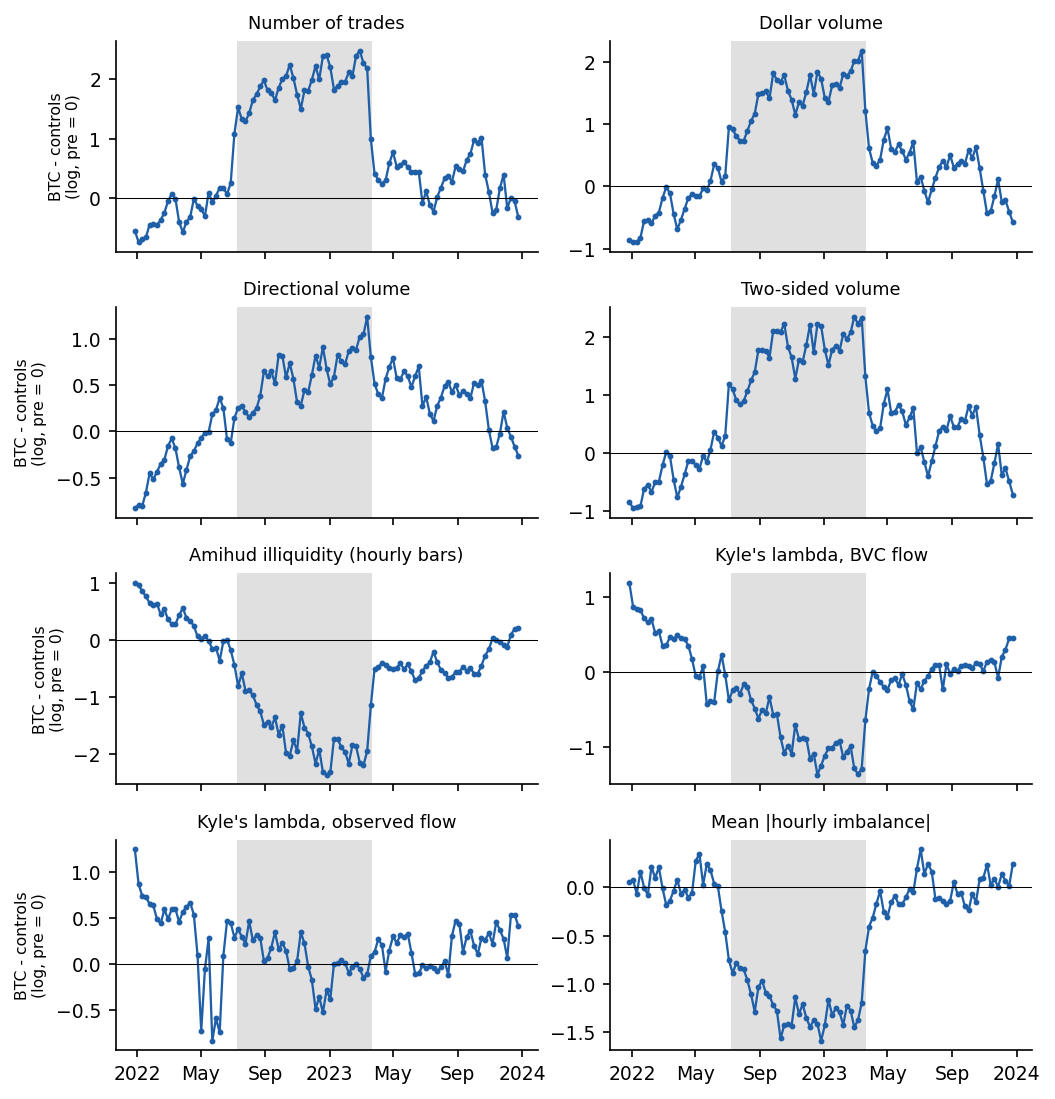
\includegraphics[width=0.95\textwidth]{fig_fee_event_study.png}
\caption{Weekly means of the BTC-minus-control difference for selected daily measures, January 2022 to
December 2023, relative to the 90 days before the promotion (log points). Shaded: zero fees on
BTC/USDT.}
\label{fig:feeevent}
\end{figure}

\section{Additional tables}

\begin{table}[H]
\centering\caption{Alternative flow classifiers vs.\ observed taker imbalance, BTC/USDT}\label{tab:variants}
\begin{tabular}{lrrrr}
\toprule
 & \multicolumn{2}{c}{Pearson} & \multicolumn{2}{c}{Same sign}\\
\cmidrule(lr){2-3}\cmidrule(lr){4-5} Classifier & 1h & 24h & 1h & 24h\\
\midrule
BVC Normal, sigma 24h (1h bars) & 0.503 & 0.516 & 0.716 & 0.695\\
BVC Normal, sigma 168h (1h bars) & 0.489 & 0.507 & 0.716 & 0.693\\
BVC Normal, sigma 720h (1h bars) & 0.484 & 0.505 & 0.716 & 0.691\\
BVC Student-t(3), sigma 168h (1h bars) & 0.494 & 0.507 & 0.716 & 0.687\\
Tick rule (1h bars) & 0.430 & 0.456 & 0.716 & 0.666\\
BVC Normal, sigma 1440m (1m bars) & 0.603 & 0.602 & 0.748 & 0.725\\
Tick rule (1m bars) & 0.597 & 0.617 & 0.728 & 0.731\\
\bottomrule
\end{tabular}

\tabnote{Correlation and sign agreement between proxy imbalance and observed taker imbalance, per hour
(1h) and over rolling 24-hour sums (24h). Student-$t$(3) is rescaled to unit variance.}
\end{table}

\begin{table}[H]
\centering\caption{Information ceiling by period}\label{tab:ceiling}
\begin{tabular}{lrrrrrr}
\toprule
Period & Hours & Ceiling & corr$^2$(BVC) & Slope & SD imb. & Ceiling (1m)\\
\midrule
\multicolumn{7}{l}{\emph{BTC/USDT}}\\
full sample & 42,315 & 0.247 & 0.239 & 0.128 & 0.130 & 0.338\\
zero-fee window & 6,154 & 0.374 & 0.360 & 0.038 & 0.030 & 0.345\\
standard fees & 36,161 & 0.267 & 0.257 & 0.142 & 0.140 & 0.362\\
2022 & 8,718 & 0.242 & 0.234 & 0.065 & 0.066 & 0.248\\
2023 & 8,757 & 0.278 & 0.253 & 0.106 & 0.099 & 0.370\\
2024 & 8,784 & 0.332 & 0.315 & 0.135 & 0.121 & 0.411\\
2025 & 8,760 & 0.281 & 0.265 & 0.167 & 0.165 & 0.362\\
2026 & 7,296 & 0.254 & 0.246 & 0.169 & 0.172 & 0.347\\
\multicolumn{7}{l}{\emph{ETH/USDT}}\\
full sample & 42,315 & 0.244 & 0.237 & 0.123 & 0.126 & 0.285\\
zero-fee window & 6,154 & 0.265 & 0.254 & 0.098 & 0.095 & 0.253\\
standard fees & 36,161 & 0.244 & 0.237 & 0.127 & 0.131 & 0.291\\
2022 & 8,718 & 0.283 & 0.275 & 0.094 & 0.091 & 0.211\\
2023 & 8,757 & 0.246 & 0.228 & 0.118 & 0.119 & 0.331\\
2024 & 8,784 & 0.319 & 0.307 & 0.129 & 0.118 & 0.336\\
2025 & 8,760 & 0.250 & 0.241 & 0.132 & 0.136 & 0.296\\
2026 & 7,296 & 0.212 & 0.199 & 0.147 & 0.163 & 0.270\\
\bottomrule
\end{tabular}

\tabnote{Ceiling: in-sample $R^2$ of observed hourly taker imbalance on 50 quantile-bin means of the
standardised bar return, the upper bound for any return-based classifier calibrated to that period.
corr$^2$(BVC): squared correlation of hourly BVC with observed imbalance. Slope: OLS slope of observed
imbalance on BVC (its calibration). SD imb.: standard deviation of observed hourly imbalance. Ceiling
(1m): the same bound for one-minute imbalance on one-minute returns.}
\end{table}

\begin{table}[H]
\centering\caption{BVC accuracy by regime, BTC/USDT}\label{tab:regimes}
\begin{tabular}{llrrrrr}
\toprule
 & & \multicolumn{2}{c}{Pearson} & \multicolumn{2}{c}{Same sign} & \\
\cmidrule(lr){3-4}\cmidrule(lr){5-6} Split & Group & 1h & 24h & 1h & 24h & Hours\\
\midrule
volatility & high vol & 0.499 & 0.619 & 0.715 & 0.744 & 13,119\\
volatility & low vol & 0.493 & 0.432 & 0.717 & 0.649 & 15,252\\
volatility & mid vol & 0.503 & 0.507 & 0.715 & 0.690 & 13,368\\
year & 2022 & 0.484 & 0.580 & 0.721 & 0.720 & 8,718\\
year & 2023 & 0.503 & 0.497 & 0.728 & 0.661 & 8,758\\
year & 2024 & 0.561 & 0.595 & 0.728 & 0.701 & 8,784\\
year & 2025 & 0.515 & 0.544 & 0.707 & 0.676 & 8,760\\
year & 2026 & 0.496 & 0.533 & 0.690 & 0.709 & 7,296\\
fee regime & standard fees & 0.507 & 0.524 & 0.710 & 0.693 & 36,148\\
fee regime & zero-fee promo & 0.600 & 0.595 & 0.749 & 0.690 & 6,168\\
\bottomrule
\end{tabular}

\tabnote{Volatility terciles use the 24h Garman-Klass volatility ranked against the trailing 30 days.}
\end{table}

\begin{table}[H]
\centering\caption{Rolling six-month estimation window, BTC/USDT}\label{tab:rolling}
\begin{tabular}{lrrrr}
\toprule
Model & Expanding $R^2_{OOS}$ & Rolling $R^2_{OOS}$ & Rolling CW $p$ & Rolling IC\\
\midrule
EN: TI & \ensuremath{-}0.055 & \ensuremath{-}0.411 & 0.52 & 0.001\\
EN: MS$_{\text{proxy}}$ & \ensuremath{-}0.139 & \ensuremath{-}0.379 & 0.73 & \ensuremath{-}0.007\\
EN: MS & \ensuremath{-}0.006 & \ensuremath{-}0.400 & 0.55 & \ensuremath{-}0.002\\
EN: ALL & \ensuremath{-}0.025 & \ensuremath{-}0.433 & 0.33 & \ensuremath{-}0.006\\
\bottomrule
\end{tabular}

\tabnote{Out-of-sample $R^2$ (\%) against the zero forecast with the expanding window of the main
analysis and with a six-month rolling window; Clark-West $p$-value and IC for the rolling window.}
\end{table}

\begin{table}[H]
\centering\caption{Drop-one-group ablation, full elastic net, BTC/USDT}\label{tab:dropgroup}
\begin{tabular}{lrrr}
\toprule
Group dropped & Features & $R^2_{OOS}$ (\%) & IC\\
\midrule
none (EN: ALL) & 45 & \ensuremath{-}0.025 & 0.019\\
spread impact & 41 & \ensuremath{-}0.115 & \ensuremath{-}0.004\\
order flow & 40 & \ensuremath{-}0.072 & 0.014\\
volatility & 39 & 0.021 & 0.018\\
efficiency structure & 39 & \ensuremath{-}0.169 & 0.006\\
activity & 43 & \ensuremath{-}0.045 & 0.011\\
trade level & 37 & \ensuremath{-}0.125 & 0.005\\
intrahour 1m & 41 & \ensuremath{-}0.118 & 0.017\\
\bottomrule
\end{tabular}

\end{table}

\begin{table}[H]
\centering\caption{Conditional out-of-sample accuracy, BTC/USDT}\label{tab:conditional}
\resizebox{\textwidth}{!}{\begin{tabular}{llrrrrr}
\toprule
Split & Group & Hours & EN: TI & EN: MS & EN: ALL & EN: Flow$_{\text{taker}}$\\
\midrule
vol regime & high & 11,647 & \ensuremath{-}0.150 (0.38) & \ensuremath{-}0.029 (0.47) & \ensuremath{-}0.080 (0.36) & \ensuremath{-}0.033 (0.72)\\
vol regime & low & 13,914 & 0.042 (0.05) & \ensuremath{-}0.056 (0.46) & 0.054 (0.06) & \ensuremath{-}0.087 (0.73)\\
vol regime & mid & 12,032 & 0.035 (0.05) & 0.085 (0.03) & 0.006 (0.12) & 0.005 (0.25)\\
illiq regime & high & 12,524 & \ensuremath{-}0.049 (0.17) & \ensuremath{-}0.026 (0.39) & 0.056 (0.12) & 0.002 (0.32)\\
illiq regime & low & 13,471 & 0.103 (0.03) & 0.070 (0.02) & 0.024 (0.08) & \ensuremath{-}0.043 (0.67)\\
illiq regime & mid & 11,598 & \ensuremath{-}0.254 (0.64) & \ensuremath{-}0.074 (0.65) & \ensuremath{-}0.181 (0.55) & \ensuremath{-}0.072 (0.85)\\
session & Asia 00-08 & 12,528 & \ensuremath{-}0.166 (0.33) & \ensuremath{-}0.086 (0.58) & \ensuremath{-}0.355 (0.73) & 0.002 (0.19)\\
session & Europe 08-16 & 12,533 & 0.014 (0.14) & 0.083 (0.03) & 0.134 (0.02) & \ensuremath{-}0.053 (0.83)\\
session & US 16-24 & 12,532 & \ensuremath{-}0.077 (0.23) & \ensuremath{-}0.076 (0.66) & \ensuremath{-}0.026 (0.23) & \ensuremath{-}0.038 (0.61)\\
weekend & weekday & 26,867 & \ensuremath{-}0.050 (0.13) & \ensuremath{-}0.005 (0.24) & 0.020 (0.05) & \ensuremath{-}0.043 (0.80)\\
weekend & weekend & 10,726 & \ensuremath{-}0.085 (0.16) & \ensuremath{-}0.010 (0.27) & \ensuremath{-}0.287 (0.52) & 0.007 (0.21)\\
fee regime & standard fees & 31,483 & \ensuremath{-}0.032 (0.05) & \ensuremath{-}0.001 (0.17) & \ensuremath{-}0.026 (0.08) & \ensuremath{-}0.026 (0.52)\\
fee regime & zero-fee (BTC/USDT promo) & 6,110 & \ensuremath{-}0.137 (0.64) & \ensuremath{-}0.023 (0.92) & \ensuremath{-}0.023 (0.92) & \ensuremath{-}0.072 (0.84)\\
\bottomrule
\end{tabular}
}
\tabnote{Out-of-sample $R^2$ against zero (\%) within each group, Clark-West $p$-value in parentheses.
Volatility and illiquidity terciles rank the 24h Garman-Klass volatility and the Amihud ratio against
the trailing 30 days, so group membership is known at forecast time.}
\end{table}

\begin{table}[H]
\centering\caption{Sub-period accuracy, BTC/USDT}\label{tab:subperiods}
\resizebox{\textwidth}{!}{\begin{tabular}{lrrrrrrr}
\toprule
Sub-period & BTC ret.\ (\%) & EN: TI & EN: MS$_{\text{proxy}}$ & EN: MS & EN: ALL & EN: Flow$_{\text{BVC}}$ & EN: Flow$_{\text{taker}}$\\
\midrule
2022-07-10--2023-08-14 & 36 & \ensuremath{-}0.162 & \ensuremath{-}0.354 & \ensuremath{-}0.018 & \ensuremath{-}0.019 & \ensuremath{-}0.228 & \ensuremath{-}0.057\\
2023-08-14--2024-09-08 & 84 & \ensuremath{-}0.086 & \ensuremath{-}0.035 & 0.045 & 0.034 & \ensuremath{-}0.058 & \ensuremath{-}0.068\\
2024-09-08--2025-10-05 & 132 & 0.319 & \ensuremath{-}0.011 & \ensuremath{-}0.050 & \ensuremath{-}0.079 & \ensuremath{-}0.008 & \ensuremath{-}0.016\\
2025-10-05--2026-10-31 & \ensuremath{-}38 & \ensuremath{-}0.272 & \ensuremath{-}0.137 & \ensuremath{-}0.009 & \ensuremath{-}0.052 & 0.000 & 0.012\\
\bottomrule
\end{tabular}
}
\tabnote{Out-of-sample $R^2$ against zero (\%) in four equal sub-periods of the test sample, with the
BTC return over each sub-period.}
\end{table}

\begin{table}[H]
\centering\caption{Out-of-sample forecast accuracy, ETH/USDT}\label{tab:forecast_eth}
\resizebox{\textwidth}{!}{\begin{tabular}{lrrrrcrr}
\toprule
Model & $R^2_{OOS}$ vs.\ 0 (\%) & $R^2_{OOS}$ vs.\ mean (\%) & CW $t$ vs.\ 0 & IC & 95\% CI & Hit rate & Hit $t$\\
\midrule
Historical mean & \ensuremath{-}0.083 & 0.000 & -- & \ensuremath{-}0.009 & [\ensuremath{-}0.028, 0.008] & -- & --\\
EN: TI & 0.102 & 0.186 & 2.97$^{***}$ & 0.012 & [\ensuremath{-}0.003, 0.029] & 0.499 & \ensuremath{-}0.20\\
EN: MS$_{\text{proxy}}$ & \ensuremath{-}0.266 & \ensuremath{-}0.182 & \ensuremath{-}1.60$$ & \ensuremath{-}0.005 & [\ensuremath{-}0.022, 0.011] & 0.495 & \ensuremath{-}0.83\\
EN: MS & \ensuremath{-}0.335 & \ensuremath{-}0.252 & \ensuremath{-}1.72$$ & 0.003 & [\ensuremath{-}0.015, 0.020] & 0.497 & \ensuremath{-}0.46\\
EN: ALL & \ensuremath{-}0.356 & \ensuremath{-}0.273 & \ensuremath{-}1.63$$ & \ensuremath{-}0.007 & [\ensuremath{-}0.025, 0.010] & 0.491 & \ensuremath{-}1.41\\
EN: Flow$_{\text{BVC}}$ & \ensuremath{-}0.083 & 0.001 & \ensuremath{-}0.34$$ & \ensuremath{-}0.014 & [\ensuremath{-}0.031, 0.003] & 0.491 & \ensuremath{-}1.91\\
EN: Flow$_{\text{taker}}$ & \ensuremath{-}0.010 & 0.073 & 1.06$$ & 0.009 & [\ensuremath{-}0.008, 0.026] & 0.505 & 1.08\\
GBM: MS & \ensuremath{-}0.441 & \ensuremath{-}0.357 & \ensuremath{-}0.32$$ & 0.002 & [\ensuremath{-}0.016, 0.017] & 0.501 & 0.25\\
GBM: ALL & \ensuremath{-}0.478 & \ensuremath{-}0.394 & \ensuremath{-}0.62$$ & \ensuremath{-}0.016 & [\ensuremath{-}0.034, 0.001] & 0.489 & \ensuremath{-}2.93\\
\bottomrule
\end{tabular}
}
\end{table}

\begin{table}[H]
\centering\caption{Incremental predictive information, ETH/USDT}\label{tab:incremental_eth}
\resizebox{\textwidth}{!}{\begin{tabular}{llcrrrrr}
\toprule
Model & Benchmark & Nested & $R^2_{OOS}$ rel.\ (\%) & CW $t$ & CW $p$ & DM $t$ & DM $p$\\
\midrule
EN: ALL & EN: TI & yes & \ensuremath{-}0.459 & \ensuremath{-}1.09$$ & 0.861 & \ensuremath{-}2.90$^{***}$ & 0.004\\
EN: MS & EN: TI & yes & \ensuremath{-}0.438 & \ensuremath{-}0.87$$ & 0.808 & \ensuremath{-}2.64$^{***}$ & 0.008\\
EN: MS & EN: MS$_{\text{proxy}}$ & yes & \ensuremath{-}0.069 & 0.37$$ & 0.354 & \ensuremath{-}0.71$$ & 0.478\\
EN: MS$_{\text{proxy}}$ & EN: TI & yes & \ensuremath{-}0.369 & \ensuremath{-}0.47$$ & 0.682 & \ensuremath{-}2.87$^{***}$ & 0.004\\
GBM: ALL & EN: TI & yes & \ensuremath{-}0.580 & \ensuremath{-}0.36$$ & 0.639 & \ensuremath{-}2.70$^{***}$ & 0.007\\
EN: Flow$_{\text{taker}}$ & EN: Flow$_{\text{BVC}}$ & no & 0.072 & -- & -- & 1.30$$ & 0.194\\
\bottomrule
\end{tabular}
}
\end{table}

\begin{table}[H]
\centering\caption{Return response to order-flow shocks, ETH/USDT}\label{tab:response_eth}
\begin{tabular}{lrrrrrr}
\toprule
Regressor (1 SD) & $k=1$h & $k=2$h & $k=4$h & $k=8$h & $k=12$h & $k=24$h\\
\midrule
Observed taker imbalance & 0.10 & \ensuremath{-}0.53 & 0.55 & 0.61 & 0.90 & 2.68\\
 & (0.33) & (\ensuremath{-}1.14) & (0.76) & (0.53) & (0.58) & (1.21)\\
BVC imbalance & 0.56 & 0.81 & 1.85 & 3.62 & 4.58 & 3.67\\
 & (1.10) & (1.10) & (1.74) & (2.29) & (2.36) & (1.31)\\
Observed imbalance, given $z_t$ & \ensuremath{-}0.15 & \ensuremath{-}0.79 & 0.21 & \ensuremath{-}0.41 & \ensuremath{-}0.46 & 2.10\\
 & (\ensuremath{-}0.45) & (\ensuremath{-}1.55) & (0.26) & (\ensuremath{-}0.31) & (\ensuremath{-}0.26) & (0.81)\\
Bar return $z_t$, given imbalance & 0.58 & 0.62 & 0.80 & 2.39 & 3.21 & 1.36\\
 & (1.10) & (0.85) & (0.76) & (1.61) & (1.69) & (0.51)\\
\bottomrule
\end{tabular}

\end{table}

\begin{table}[H]
\centering\caption{Proxy validation, ETH/USDT}\label{tab:validation_eth}
\resizebox{\textwidth}{!}{\begin{tabular}{lrrrr}
\toprule
 & Pearson & Spearman & Same sign & $N$\\
\midrule
\multicolumn{5}{l}{\emph{Panel A. Signed order flow: proxy vs.\ observed taker imbalance}}\\
BVC, 1h bars, per hour & 0.487 & 0.532 & 0.708 & 42,316\\
BVC, 1h bars, 4h sums & 0.470 & 0.530 & 0.708 & 42,310\\
BVC, 1h bars, 24h sums & 0.513 & 0.561 & 0.720 & 42,270\\
BVC, 1m bars summed to 1h & 0.556 & 0.605 & 0.735 & 42,359\\
Tick rule, 1h bars, per hour & 0.432 & 0.418 & 0.708 & 42,357\\
\midrule
\multicolumn{5}{l}{\emph{Panel B. Price impact and volatility}}\\
Kyle $\lambda$ (48h): BVC vs.\ observed flow & 0.440 & 0.503 & -- & 41,978\\
log GK vol (1h bars) vs.\ log RV (1m), 24h & 0.987 & 0.984 & -- & 41,978\\
\midrule
\multicolumn{5}{l}{\emph{Panel C. Information ceiling of return-based classifiers (out-of-sample $R^2$)}}\\
 & BVC raw & BVC rescaled & Any $f(z)$ & $N$\\
1h bars & \ensuremath{-}8.868 & 0.218 & 0.222 & 21,158\\
1m bars & \ensuremath{-}0.153 & 0.276 & 0.286 & 1,270,544\\
\midrule
\multicolumn{5}{l}{\emph{Panel D. Spread estimators (one tick $=$ 0.043 bps)}}\\
 & Median (bps) & Mean (bps) & Share $=0$ & Corr.\ log RV\\
Corwin-Schultz (24h mean) & 20.7 & 23.2 & 0.0\% & 0.85\\
Abdi-Ranaldo (24h) & 0.0 & 11.1 & 54.7\% & 0.61\\
Roll (48h) & 17.6 & 24.0 & 40.6\% & 0.52\\
\bottomrule
\end{tabular}
}
\end{table}

\begin{table}[H]
\centering\caption{BVC accuracy by regime, ETH/USDT}\label{tab:regimes_eth}
\begin{tabular}{llrrrrr}
\toprule
 & & \multicolumn{2}{c}{Pearson} & \multicolumn{2}{c}{Same sign} & \\
\cmidrule(lr){3-4}\cmidrule(lr){5-6} Split & Group & 1h & 24h & 1h & 24h & Hours\\
\midrule
volatility & high vol & 0.500 & 0.585 & 0.714 & 0.745 & 13,547\\
volatility & low vol & 0.478 & 0.468 & 0.697 & 0.699 & 15,050\\
volatility & mid vol & 0.510 & 0.541 & 0.715 & 0.717 & 13,142\\
year & 2022 & 0.525 & 0.666 & 0.713 & 0.758 & 8,718\\
year & 2023 & 0.478 & 0.462 & 0.700 & 0.678 & 8,758\\
year & 2024 & 0.554 & 0.575 & 0.727 & 0.733 & 8,784\\
year & 2025 & 0.491 & 0.541 & 0.703 & 0.725 & 8,760\\
year & 2026 & 0.446 & 0.477 & 0.693 & 0.701 & 7,296\\
fee regime & standard fees & 0.487 & 0.515 & 0.708 & 0.723 & 36,162\\
fee regime & zero-fee promo & 0.504 & 0.571 & 0.710 & 0.700 & 6,154\\
\bottomrule
\end{tabular}

\end{table}
